% Name: Floating block
% Description: A block floating in water with 60% of its height submerged: its weight and the equal buoyant force, the submerged depth d, and the height h.
% Tags: buoyancy, Archimedes' principle, fluids, density

\usetikzlibrary{arrows.meta}

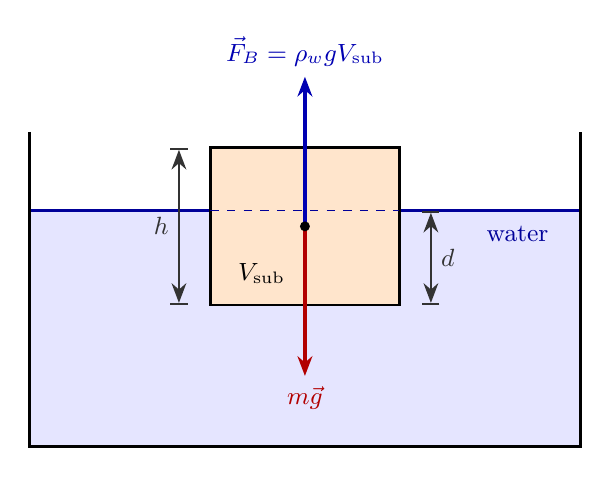
\begin{tikzpicture}[>={Stealth[length=2.5mm]}, force/.style={->, very thick}, every node/.style={font=\small}]
  % Floating: rho_block h = rho_water d, so a block 0.6 as dense as water sinks to d = 0.6 h = 1.2 of h = 2.
  \fill[blue!10] (0,0) rectangle (7,3);
  \draw[blue!60!black, thick] (0,3) -- (2.3,3) (4.7,3) -- (7,3);
  \draw[very thick] (0,4) -- (0,0) -- (7,0) -- (7,4);
  \draw[thick, fill=orange!20] (2.3,1.8) rectangle (4.7,3.8);
  \draw[dashed, blue!60!black] (2.3,3) -- (4.7,3);
  \node[blue!60!black] at (6.2,2.7) {water};
  \node at (2.95,2.2) {$V_{\mathrm{sub}}$};
  \coordinate (G) at (3.5,2.8);
  \draw[force, blue!70!black] (G) -- ++(0,1.9) node[above] {$\vec{F}_B = \rho_w g V_{\mathrm{sub}}$};
  \draw[force, red!70!black] (G) -- ++(0,-1.9) node[below] {$m\vec{g}$};
  \fill (G) circle (1.8pt);
  \draw[|<->|, thick, gray!40!black] (5.1,1.8) -- node[right] {$d$} (5.1,3);
  \draw[|<->|, thick, gray!40!black] (1.9,1.8) -- node[left] {$h$} (1.9,3.8);
\end{tikzpicture}
